
\documentclass[11pt]{article}
\usepackage[margin=0.78in]{geometry}
\usepackage{booktabs}
\usepackage{longtable}
\usepackage{tabularx}
\usepackage{array}
\usepackage{graphicx}
\usepackage{float}
\usepackage{xcolor}
\usepackage{hyperref}
\usepackage{amsmath}
\usepackage{tikz}
\usetikzlibrary{arrows.meta,positioning,shapes.geometric}
\hypersetup{colorlinks=true, linkcolor=blue, urlcolor=blue}
\setlength{\parskip}{0.45em}
\setlength{\parindent}{0pt}
\renewcommand{\arraystretch}{1.15}

\title{Liquid-Exit TP2 Rebuild Report\\\large SPY Call Option TP2 Research Pipeline}
\author{ML-Based Trading of TP2-Inspired Violations in SPY American Call Options}
\date{June 21, 2026}

\begin{document}
\maketitle

\section{Purpose}

This report documents the liquid-exit rebuild of the TP2-inspired SPY call option pipeline. The
goal is to preserve the full TP2 lifecycle path while enforcing liquidity only where it matters
economically: at trade entry and trade exit. This was motivated by the observation that a TP2
violation may revert before the selected option legs are cleanly executable. The prior strict
reversion-day mini-backtest could therefore mark a trade invalid even though a realistic trader
could close it on the first later liquid date before expiration.

The rebuild is implemented as a parallel layer. It does not overwrite the earlier episode,
lifecycle, or conservative bid/ask outputs.

\section{High-Level Result}

\begin{center}
\begin{tabular}{lr}
\toprule
Quantity & Value \\
\midrule
Entry episodes & 226,577 \\
Strategy-exit-policy rows & 5,437,848 \\
Valid strategy-exit-policy rows & 2,364,690 \\
Total valid net P\&L across all implemented policies & -\$144.01M \\
Implemented strategies & T1, T2, K1, K2 \\
Implemented exit policies & 6 \\
\bottomrule
\end{tabular}
\end{center}

The main live-style policy is \texttt{exit\_first\_liquid\_on\_or\_after\_reversion}. The
expiration-payoff policy is included as a Glasserman-style benchmark, not as the same execution
question as premium resale.

\section{Pipeline From Zero}

\begin{figure}[H]
\centering
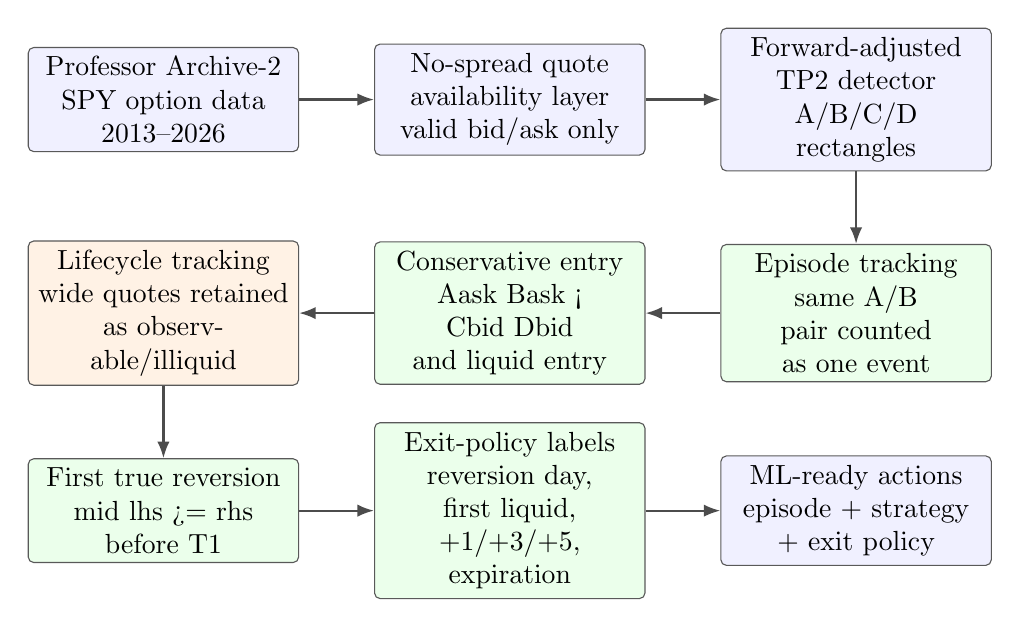
\begin{tikzpicture}[
  node distance=0.92cm and 0.95cm,
  box/.style={rectangle, rounded corners=2pt, draw=black!65, fill=blue!6, text width=3.2cm, align=center, minimum height=0.9cm},
  good/.style={rectangle, rounded corners=2pt, draw=black!65, fill=green!8, text width=3.2cm, align=center, minimum height=0.9cm},
  warn/.style={rectangle, rounded corners=2pt, draw=black!65, fill=orange!10, text width=3.2cm, align=center, minimum height=0.9cm},
  arrow/.style={-{Latex[length=2.1mm]}, thick, draw=black!70}
]
\node[box] (raw) {Professor Archive-2\\SPY option data\\2013--2026};
\node[box, right=of raw] (quote) {No-spread quote\\availability layer\\valid bid/ask only};
\node[box, right=of quote] (tp2) {Forward-adjusted\\TP2 detector\\A/B/C/D rectangles};
\node[good, below=of tp2] (episode) {Episode tracking\\same A/B pair counted\\as one event};
\node[good, left=of episode] (entry) {Conservative entry\\Aask Bask < Cbid Dbid\\and liquid entry};
\node[warn, left=of entry] (life) {Lifecycle tracking\\wide quotes retained\\as observable/illiquid};
\node[good, below=of life] (rev) {First true reversion\\mid lhs >= rhs\\before T1};
\node[good, right=of rev] (exit) {Exit-policy labels\\reversion day, first liquid,\\+1/+3/+5, expiration};
\node[box, right=of exit] (ml) {ML-ready actions\\episode + strategy\\+ exit policy};

\draw[arrow] (raw) -- (quote);
\draw[arrow] (quote) -- (tp2);
\draw[arrow] (tp2) -- (episode);
\draw[arrow] (episode) -- (entry);
\draw[arrow] (entry) -- (life);
\draw[arrow] (life) -- (rev);
\draw[arrow] (rev) -- (exit);
\draw[arrow] (exit) -- (ml);
\end{tikzpicture}
\caption{Liquid-exit rebuild architecture. Liquidity is stored throughout, but enforced only when opening or closing a trade.}
\end{figure}

\subsection{Data Layer}

The rebuild uses the no-spread quote availability file:

\begin{quote}\small
\texttt{data/processed/archive2\_spy\_call\_quote\_availability\_nospread\_2013\_2026.parquet}
\end{quote}

This file keeps SPY calls with valid bid/ask, positive bid, positive mid, and the latest available
contract-day quote. It also applies a broad call-price sanity filter:

\[
\max(S-K,0)-1 \le C_{mid} \le 1.05S+1.
\]

This removes raw vendor artifacts where a deep in-the-money call is priced far below intrinsic
value or above the underlying itself. It is not a model fit; it is a static no-arbitrage data
quality screen. The file does not delete rows solely because the bid/ask spread exceeds 50\%.
Instead it stores \texttt{spread\_pct}, \texttt{tradable\_under\_50pct\_spread}, and
\texttt{wide\_spread\_over\_50pct}. This is the key structural correction: wide quotes remain
available for behavior tracking but cannot be used as executable fills.

\subsection{TP2 Rectangle And Violation Definitions}

For calls, each rectangle contains:

\begin{align*}
A &= C(K_1,T_1), & B &= C(K_2,T_2),\\
C &= C(\tilde K_1,T_2), & D &= C(\tilde K_2,T_1),
\end{align*}

where the right-side strikes are forward-adjusted and rounded up to available strikes. The
mid-price TP2 pressure is:

\[
\text{pressure} = C_{mid}D_{mid} - A_{mid}B_{mid}.
\]

Positive pressure means a TP2 violation. The conservative tradable entry condition is stricter:

\[
A_{ask}B_{ask} < C_{bid}D_{bid}.
\]

This means the violation survives the unfavorable side of the bid/ask spread.

\subsection{Episode Tracking}

Daily violations are grouped by the same left-side economic pair:

\begin{quote}\small
\texttt{pair\_key = A\_expiration | A\_strike | B\_expiration | B\_strike}
\end{quote}

The same continuing violation is therefore counted once as an episode, not repeatedly every day.
The liquid-exit rebuild starts from conservative bid/ask episode starts that were executable at
entry.

\subsection{Lifecycle And Reversion Tracking}

For each entry episode, the lifecycle panel tracks the same A/B pair from 20 sessions before the
first violation through T1 expiration. On each lifecycle date, the pipeline reconstructs C/D using
the current forward adjustment and round-up strike rule. Reversion is defined as the first later
date where:

\[
A_{mid}B_{mid} \ge C_{mid}D_{mid}.
\]

The important point is that reversion is measured in the no-spread quote availability universe.
If a row is observable but wide, it is still useful for identifying the TP2 path. It is not
automatically an executable exit.

\subsection{Strategy Sizing And Execution}

The rebuild uses product-weighted Glasserman-style quantities. For calls:

\begin{center}
\begin{tabular}{lll}
\toprule
Strategy & Long leg & Short leg \\
\midrule
T1 & B\_mid units of A & C\_mid units of D \\
T2 & A\_mid units of B & D\_mid units of C \\
K1 & B\_mid units of A & D\_mid units of C \\
K2 & A\_mid units of B & C\_mid units of D \\
\bottomrule
\end{tabular}
\end{center}

Execution is bid/ask based. Long positions are opened at ask and closed at bid. Short positions
are opened at bid and closed at ask. Transaction cost is \$0.65 per contract per side.

\section{Exit Policies Implemented}

\begin{center}
\begin{tabularx}{0.96\linewidth}{lX}
\toprule
Exit policy & Interpretation \\
\midrule
\texttt{exit\_at\_reversion\_day} & Strict close on the first TP2 reversion date. Selected legs must be liquid that same day. \\
\texttt{exit\_first\_liquid\_on\_or\_after\_reversion} & Main live-style policy. If reversion day is not executable, wait for the first later liquid selected-leg close before selected-leg expiration. \\
\texttt{exit\_reversion\_plus\_1\_session} & Robustness policy: exit one trading session after reversion. \\
\texttt{exit\_reversion\_plus\_3\_sessions} & Robustness policy: exit three trading sessions after reversion. \\
\texttt{exit\_reversion\_plus\_5\_sessions} & Robustness policy: exit five trading sessions after reversion. \\
\texttt{exit\_selected\_leg\_expiration\_payoff} & Glasserman-style benchmark using expiration payoff of selected legs. This is a benchmark, not the same premium-resale execution question. \\
\bottomrule
\end{tabularx}
\end{center}

\section{Main Live-Style Policy Results}

\begin{center}
\begin{tabular}{lrrrrrr}
\toprule
strategy & valid & valid\_rate & hit\_rate & net\_pnl & median\_return & mean\_holding\_days \\
\midrule
K1 & 106,232 & 46.89\% & 25.84\% & -\$19.40M & -2.48\% & 2.63 \\
K2 & 83,703 & 36.94\% & 30.49\% & -\$24.42M & -1.93\% & 2.73 \\
T1 & 83,846 & 37.01\% & 37.58\% & -\$49.09M & -2.27\% & 2.73 \\
T2 & 101,337 & 44.73\% & 31.84\% & -\$3.34M & -3.09\% & 2.70 \\
\bottomrule
\end{tabular}
\end{center}

For the first-liquid-after-reversion policy, T1 and K1 remain the main positive aggregate
strategies. The valid row count is slightly higher than strict reversion-day exit, confirming that
some episodes revert before the selected legs are immediately executable. However, the total P\&L
is close to the strict rule, so the main value of the liquid-exit correction is methodological
cleanliness and executable coverage rather than a dramatic profit change.

\subsection{Why Median Return Is Often Negative}

Median return is the middle trade return after sorting all valid strategy-policy rows. If the median
return is negative, more than half of the individual trades lose money. This can happen at the
same time that total net P\&L is strongly positive because product-weighted option strategies have
highly skewed payoffs: many small/medium losses can be outweighed by a smaller number of very
large winners.

That is exactly why the unconditional pipeline should not be the final trading rule. TP2 gives a
theoretically motivated candidate set, but the ML layer is needed to select which episodes, strategy
denominations, and exit policies are worth trading. In short: positive total P\&L with negative median
return means the signal has useful tails, but needs selection.

\section{Year-Wise Interpretation For The Main Live-Style Policy}

\small
\begin{longtable}{llllp{5.2cm}}
\toprule
Year & K1 P\&L & T1 P\&L & Valid K1/T1 & Interpretation \\
\midrule
\endfirsthead
\toprule
Year & K1 P\&L & T1 P\&L & Valid K1/T1 & Interpretation \\
\midrule
\endhead
2013 & -\$9.43M & -\$31.07M & 16,827/16,826 & Negative aggregate year; unconditional trading is weak and supports ML filtering. \\
2014 & -\$37 & -\$6 & 46/5 & Small economic contribution; useful mainly for sample coverage and robustness. \\
2015 & -\$655 & \$530 & 49/12 & Small economic contribution; useful mainly for sample coverage and robustness. \\
2016 & -\$43.0K & -\$127.9K & 1,814/1,238 & Small economic contribution; useful mainly for sample coverage and robustness. \\
2017 & -\$7.30M & -\$8.37M & 10,004/9,337 & Negative aggregate year; unconditional trading is weak and supports ML filtering. \\
2018 & -\$135.0K & \$2.03M & 3,373/3,105 & Positive aggregate year, but still heterogeneous across strategies. \\
2019 & -\$204.6K & \$4.22M & 3,327/3,055 & Positive aggregate year, but still heterogeneous across strategies. \\
2020 & -\$3.28M & -\$9.61M & 23,260/22,533 & High reversion coverage but negative T1/K1 P\&L, consistent with stressed COVID-period option repricing overwhelming simple reversion exits. \\
2021 & -\$1.06M & -\$5.63M & 11,035/7,695 & Negative aggregate year; unconditional trading is weak and supports ML filtering. \\
2022 & -\$79.5K & \$3.5K & 3,668/2,338 & Small economic contribution; useful mainly for sample coverage and robustness. \\
2023 & -\$5.9K & -\$962.5K & 4,710/2,785 & Small economic contribution; useful mainly for sample coverage and robustness. \\
2024 & -\$93.4K & -\$28.5K & 11,470/6,559 & Many valid episodes; 2025 turns positive while 2024 is mildly negative, so recent data still needs ML selection rather than unconditional trading. \\
2025 & \$2.13M & \$556.5K & 14,557/7,339 & Positive aggregate year, but still heterogeneous across strategies. \\
2026 & \$101.7K & -\$107.8K & 2,092/1,019 & Small economic contribution; useful mainly for sample coverage and robustness. \\
\bottomrule
\end{longtable}
\normalsize

The year-wise pattern confirms that unconditional TP2 trading is not uniformly profitable. The
main research value is the labeled action dataset: it lets ML learn when the TP2 dislocation is
tradable and which strategy/exit rule should be selected.

\section{All Exit Policies}

\begin{center}
\begin{tabularx}{0.96\linewidth}{lX}
\toprule
Short label & Full policy \\
\midrule
\texttt{rev-day} & \texttt{exit\_at\_reversion\_day} \\
\texttt{first-liquid} & \texttt{exit\_first\_liquid\_on\_or\_after\_reversion} \\
\texttt{rev+1} & \texttt{exit\_reversion\_plus\_1\_session} \\
\texttt{rev+3} & \texttt{exit\_reversion\_plus\_3\_sessions} \\
\texttt{rev+5} & \texttt{exit\_reversion\_plus\_5\_sessions} \\
\texttt{expiration} & \texttt{exit\_selected\_leg\_expiration\_payoff} \\
\bottomrule
\end{tabularx}
\end{center}

\begin{center}
\footnotesize
\begin{tabular}{llrrrrr}
\toprule
Policy & Strat. & Valid & Hit rate & Net P\&L & Med. ret. & Hold days \\
\midrule
rev-day & K1 & 105,591 & 25.86\% & -\$19.35M & -2.46\% & 2.62 \\
rev-day & K2 & 79,965 & 30.88\% & -\$24.58M & -1.78\% & 2.57 \\
rev-day & T1 & 80,226 & 37.85\% & -\$49.16M & -2.12\% & 2.58 \\
rev-day & T2 & 100,685 & 31.84\% & -\$3.26M & -3.08\% & 2.69 \\
first-liquid & K1 & 106,232 & 25.84\% & -\$19.40M & -2.48\% & 2.63 \\
first-liquid & K2 & 83,703 & 30.49\% & -\$24.42M & -1.93\% & 2.73 \\
first-liquid & T1 & 83,846 & 37.58\% & -\$49.09M & -2.27\% & 2.73 \\
first-liquid & T2 & 101,337 & 31.84\% & -\$3.34M & -3.09\% & 2.70 \\
rev+1 & K1 & 93,864 & 28.29\% & -\$21.77M & -1.47\% & 3.93 \\
rev+1 & K2 & 71,366 & 44.33\% & -\$2.15M & -0.85\% & 3.82 \\
rev+1 & T1 & 71,746 & 56.06\% & -\$5.41M & 1.00\% & 3.83 \\
rev+1 & T2 & 98,279 & 29.39\% & -\$25.67M & -3.87\% & 3.98 \\
rev+3 & K1 & 75,827 & 29.08\% & -\$13.85M & -1.60\% & 6.66 \\
rev+3 & K2 & 60,789 & 46.70\% & -\$7.38M & -0.54\% & 6.50 \\
rev+3 & T1 & 60,986 & 52.41\% & -\$22.54M & 0.52\% & 6.51 \\
rev+3 & T2 & 91,832 & 37.59\% & -\$4.17M & -2.46\% & 6.85 \\
rev+5 & K1 & 57,898 & 33.88\% & -\$10.75M & -0.98\% & 9.65 \\
rev+5 & K2 & 48,488 & 48.55\% & -\$10.64M & -0.18\% & 9.54 \\
rev+5 & T1 & 48,826 & 61.36\% & -\$17.30M & 2.43\% & 9.55 \\
rev+5 & T2 & 83,312 & 34.57\% & -\$27.25M & -3.52\% & 9.92 \\
expiration & K1 & 177,943 & 68.78\% & -\$118.56M & 6.58\% & 26.42 \\
expiration & K2 & 177,943 & 27.95\% & \$173.84M & -17.89\% & 26.42 \\
expiration & T1 & 188,077 & 27.17\% & -\$32.16M & -17.55\% & 12.53 \\
expiration & T2 & 215,929 & 70.87\% & \$194.35M & 6.85\% & 28.59 \\
\bottomrule
\end{tabular}
\normalsize
\end{center}

Every policy-strategy row starts from the same 226,577 selected entry episodes; the table reports how many rows remain executable under each exit rule.

\section{Expiration-Payoff Benchmark}

\begin{center}
\begin{tabular}{lrrrrr}
\toprule
strategy & valid & hit\_rate & net\_pnl & median\_return & mean\_holding\_days \\
\midrule
K1 & 177,943 & 68.78\% & -\$118.56M & 6.58\% & 26.42 \\
K2 & 177,943 & 27.95\% & \$173.84M & -17.89\% & 26.42 \\
T1 & 188,077 & 27.17\% & -\$32.16M & -17.55\% & 12.53 \\
T2 & 215,929 & 70.87\% & \$194.35M & 6.85\% & 28.59 \\
\bottomrule
\end{tabular}
\end{center}

The expiration payoff benchmark answers a different question from the liquid-exit premium-resale
rules. It is useful because Glasserman-style strategy evaluation often holds option legs to
expiration, while the live-style pipeline asks whether the premium trade can be closed after the
violation reverts.

\section{Reversion And Exit Availability}

\begin{center}
\begin{tabular}{lrrrrr}
\toprule
strategy & valid & same\_day\_exit & same\_day\_exit\_share & median\_wait\_days & p90\_wait\_days \\
\midrule
K1 & 106,232 & 105,591 & 99.40\% & 0.0 & 0.0 \\
K2 & 83,703 & 79,965 & 95.53\% & 0.0 & 0.0 \\
T1 & 83,846 & 80,226 & 95.68\% & 0.0 & 0.0 \\
T2 & 101,337 & 100,685 & 99.36\% & 0.0 & 0.0 \\
\bottomrule
\end{tabular}
\end{center}

Most first-liquid exits occur on the same calendar day as reversion. T1 and K2 still gain thousands
of additional executable rows relative to strict reversion-day exit, which is exactly why the
liquid-exit rule is worth keeping: it avoids rejecting trades only because the exact reversion day
was not executable.

\begin{center}
\begin{tabular}{rrrrrr}
\toprule
Year & Episodes & Reverted & Revert share & Med day & P75 day \\
\midrule
2013 & 49,090 & 16,827 & 34.28\% & 1.0 & 1.0 \\
2014 & 438 & 46 & 10.50\% & 1.0 & 4.0 \\
2015 & 140 & 49 & 35.00\% & 3.0 & 5.0 \\
2016 & 3,786 & 1,815 & 47.94\% & 2.0 & 3.0 \\
2017 & 12,284 & 10,004 & 81.44\% & 1.0 & 1.0 \\
2018 & 5,969 & 3,381 & 56.64\% & 1.0 & 1.0 \\
2019 & 4,151 & 3,327 & 80.15\% & 1.0 & 1.0 \\
2020 & 25,717 & 23,299 & 90.60\% & 1.0 & 1.0 \\
2021 & 20,588 & 11,044 & 53.64\% & 1.0 & 1.0 \\
2022 & 6,604 & 3,675 & 55.65\% & 1.0 & 1.0 \\
2023 & 12,731 & 4,893 & 38.43\% & 1.0 & 2.0 \\
2024 & 34,167 & 12,054 & 35.28\% & 2.0 & 3.0 \\
2025 & 41,577 & 16,874 & 40.58\% & 1.0 & 2.0 \\
2026 & 9,335 & 2,458 & 26.33\% & 1.0 & 2.0 \\
\bottomrule
\end{tabular}
\end{center}

\section{Visual Diagnostics}


\begin{figure}[H]
  \centering
  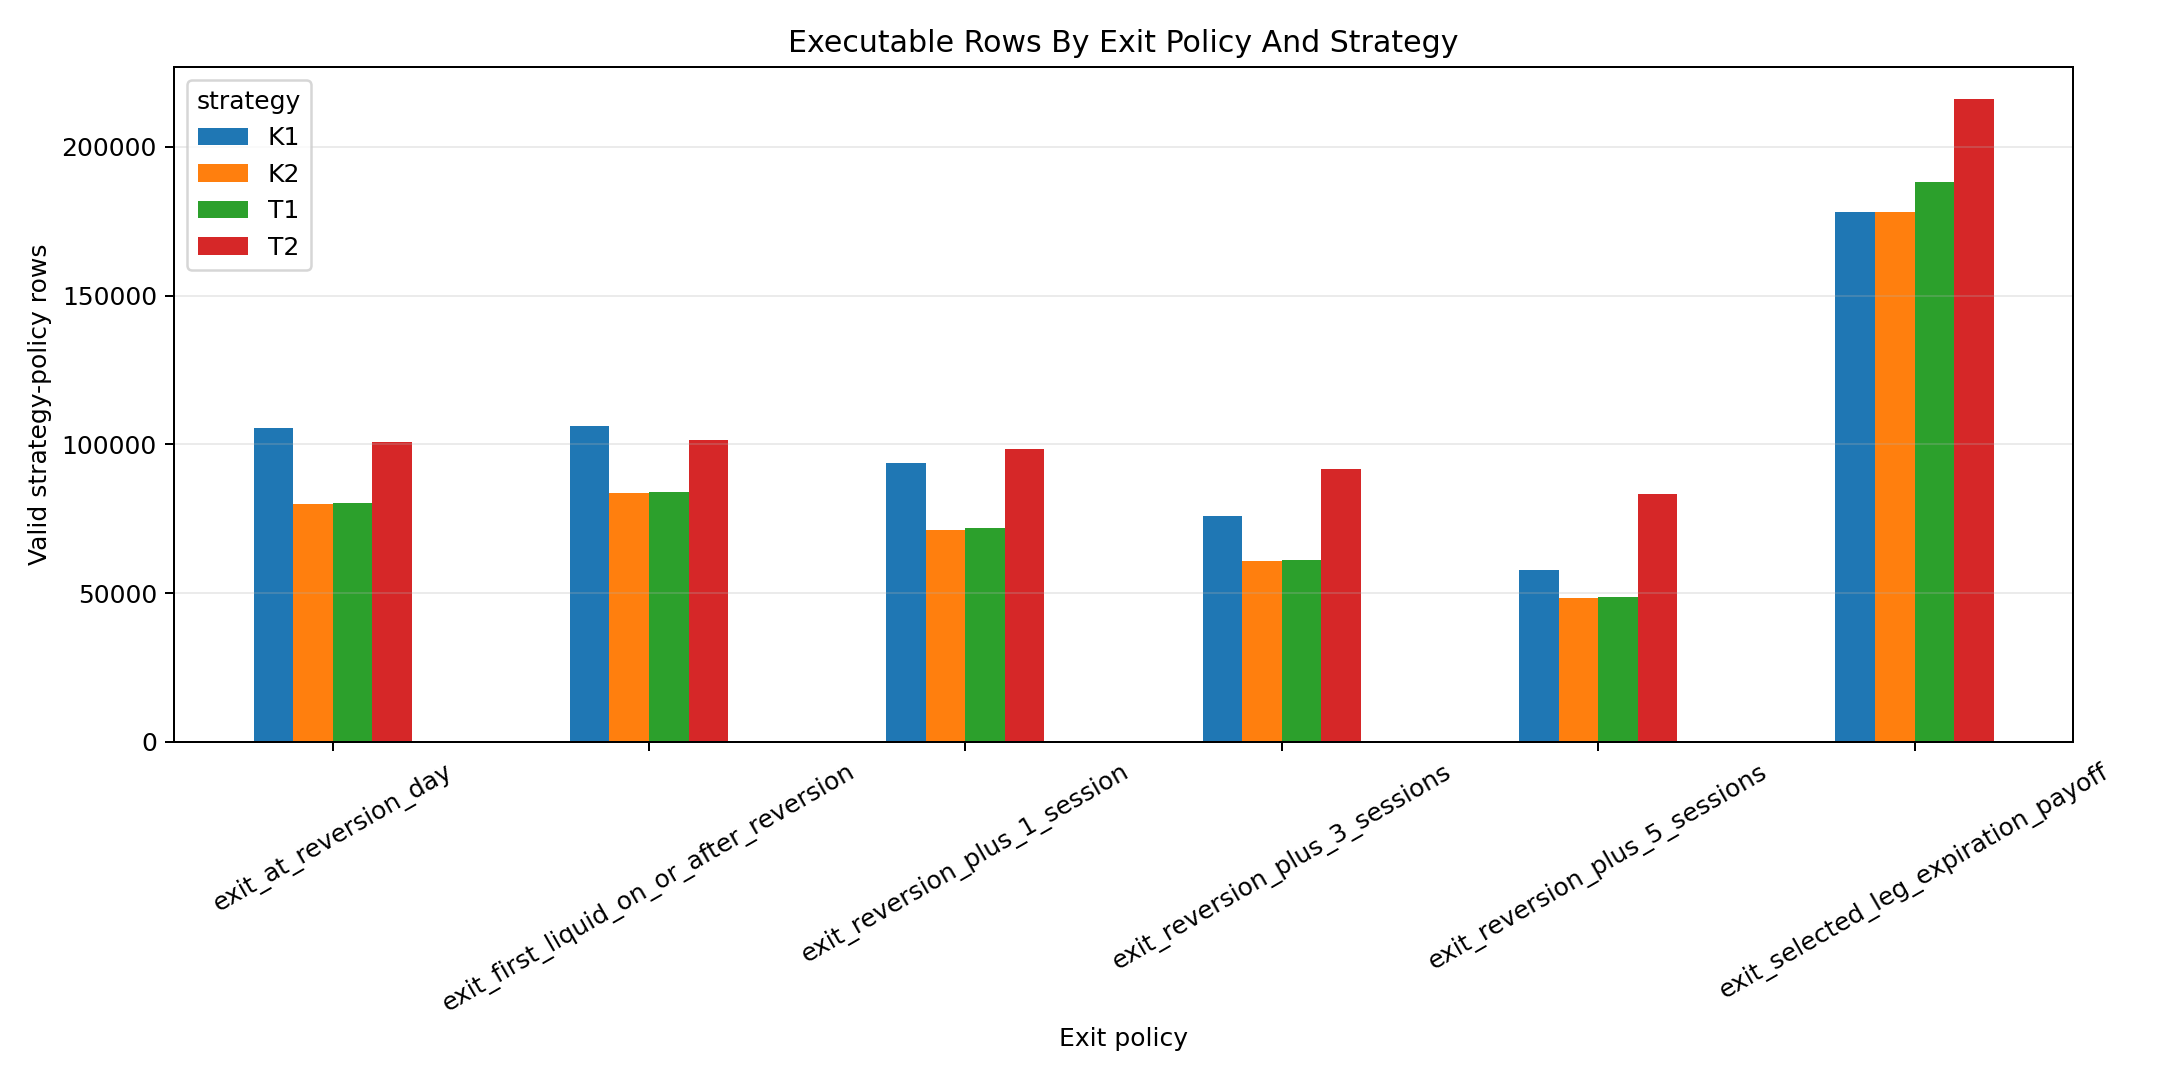
\includegraphics[width=0.92\linewidth]{figures/liquid_exit_valid_rows_by_policy_strategy.png}
  \caption{Executable rows by exit policy and strategy. First-liquid-after-reversion increases valid rows over strict reversion-day exit for several strategies.}
  \label{fig:valid_rows}
\end{figure}



\begin{figure}[H]
  \centering
  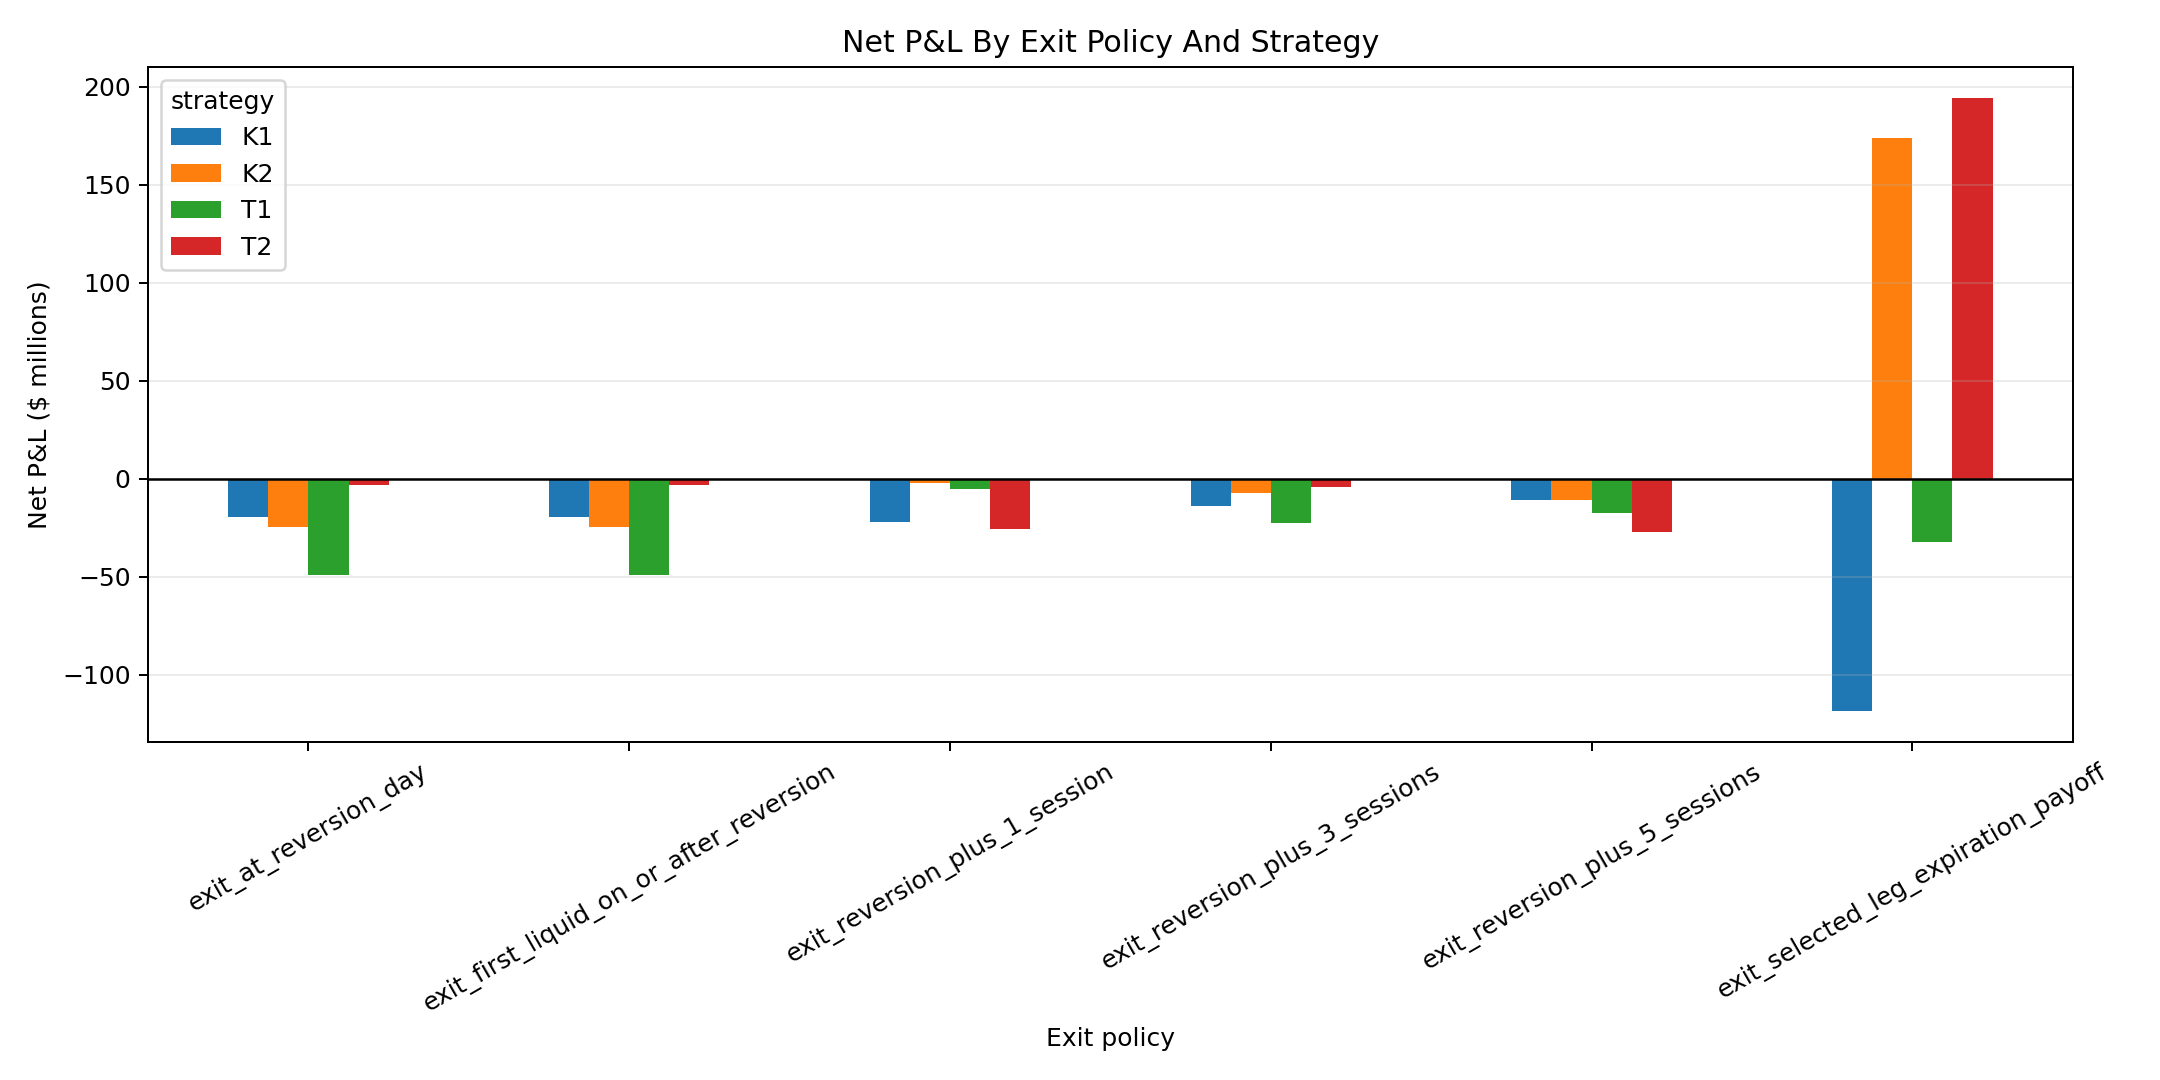
\includegraphics[width=0.92\linewidth]{figures/liquid_exit_net_pnl_by_policy_strategy.png}
  \caption{Net P\&L by exit policy and strategy. T1 and K1 dominate the live-style premium-resale policies in aggregate.}
  \label{fig:pnl_policy}
\end{figure}



\begin{figure}[H]
  \centering
  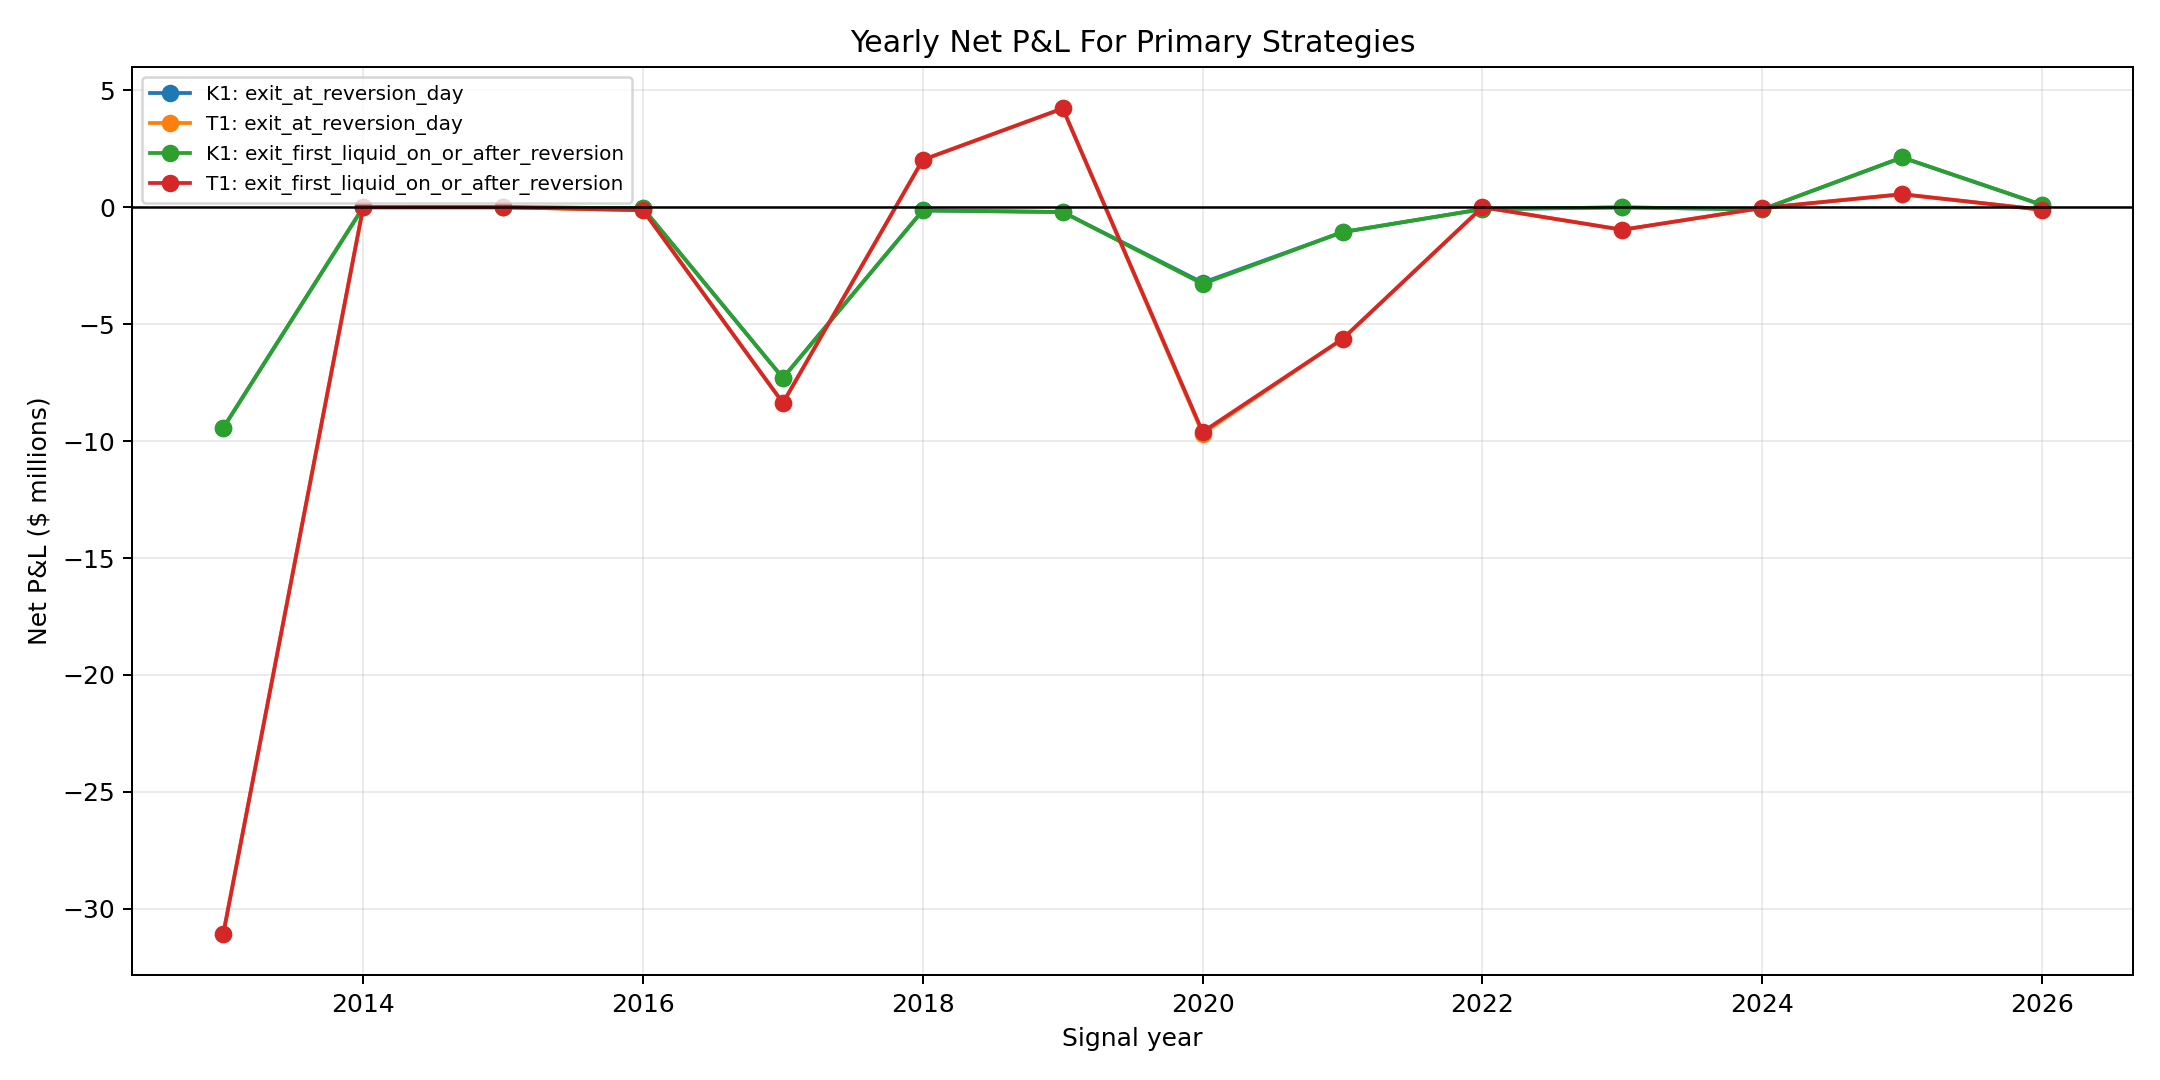
\includegraphics[width=0.92\linewidth]{figures/liquid_exit_yearly_primary_pnl.png}
  \caption{Yearly net P\&L for T1 and K1 under strict reversion-day and first-liquid-after-reversion exits.}
  \label{fig:yearly_pnl}
\end{figure}



\begin{figure}[H]
  \centering
  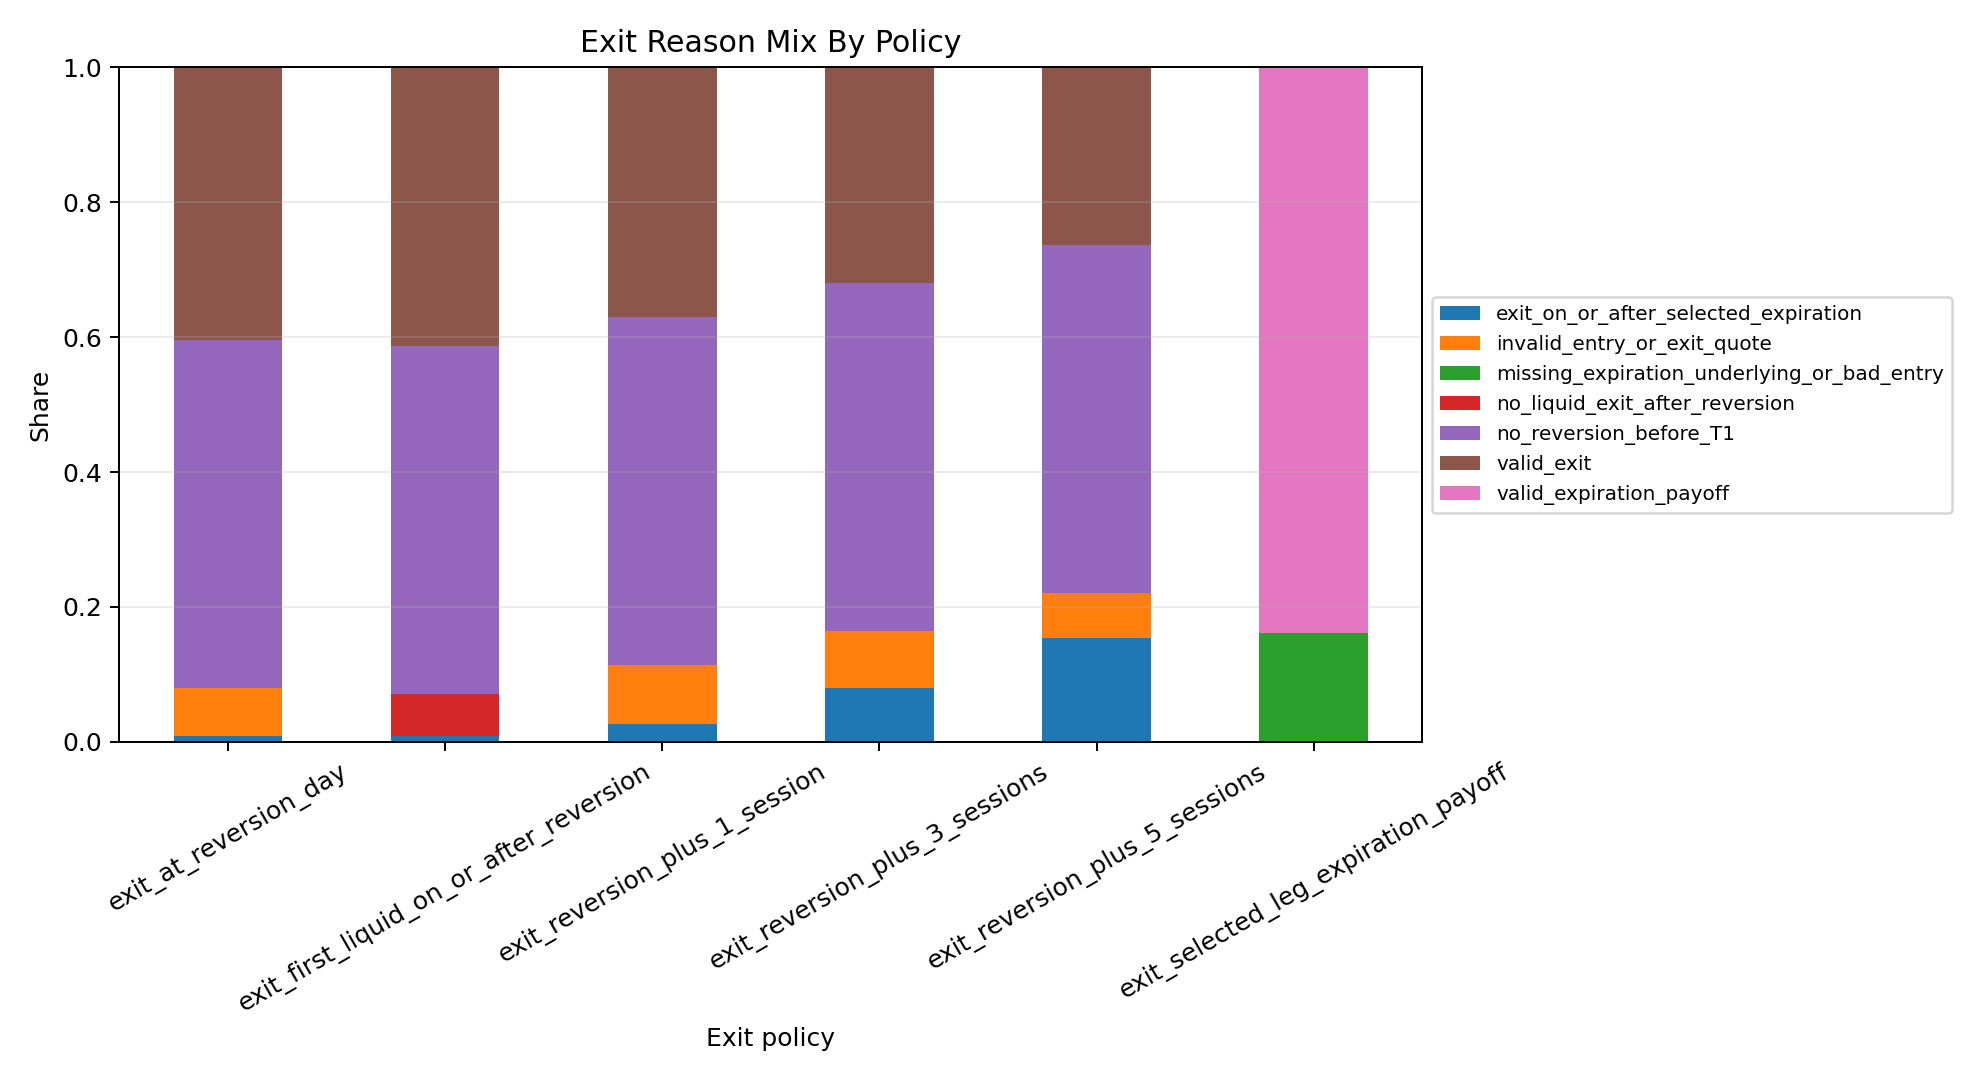
\includegraphics[width=0.92\linewidth]{figures/liquid_exit_reason_mix_by_policy.png}
  \caption{Exit reason mix by policy. No-reversion and invalid/late exits are retained in accounting rather than silently removed.}
  \label{fig:reason_mix}
\end{figure}



\begin{figure}[H]
  \centering
  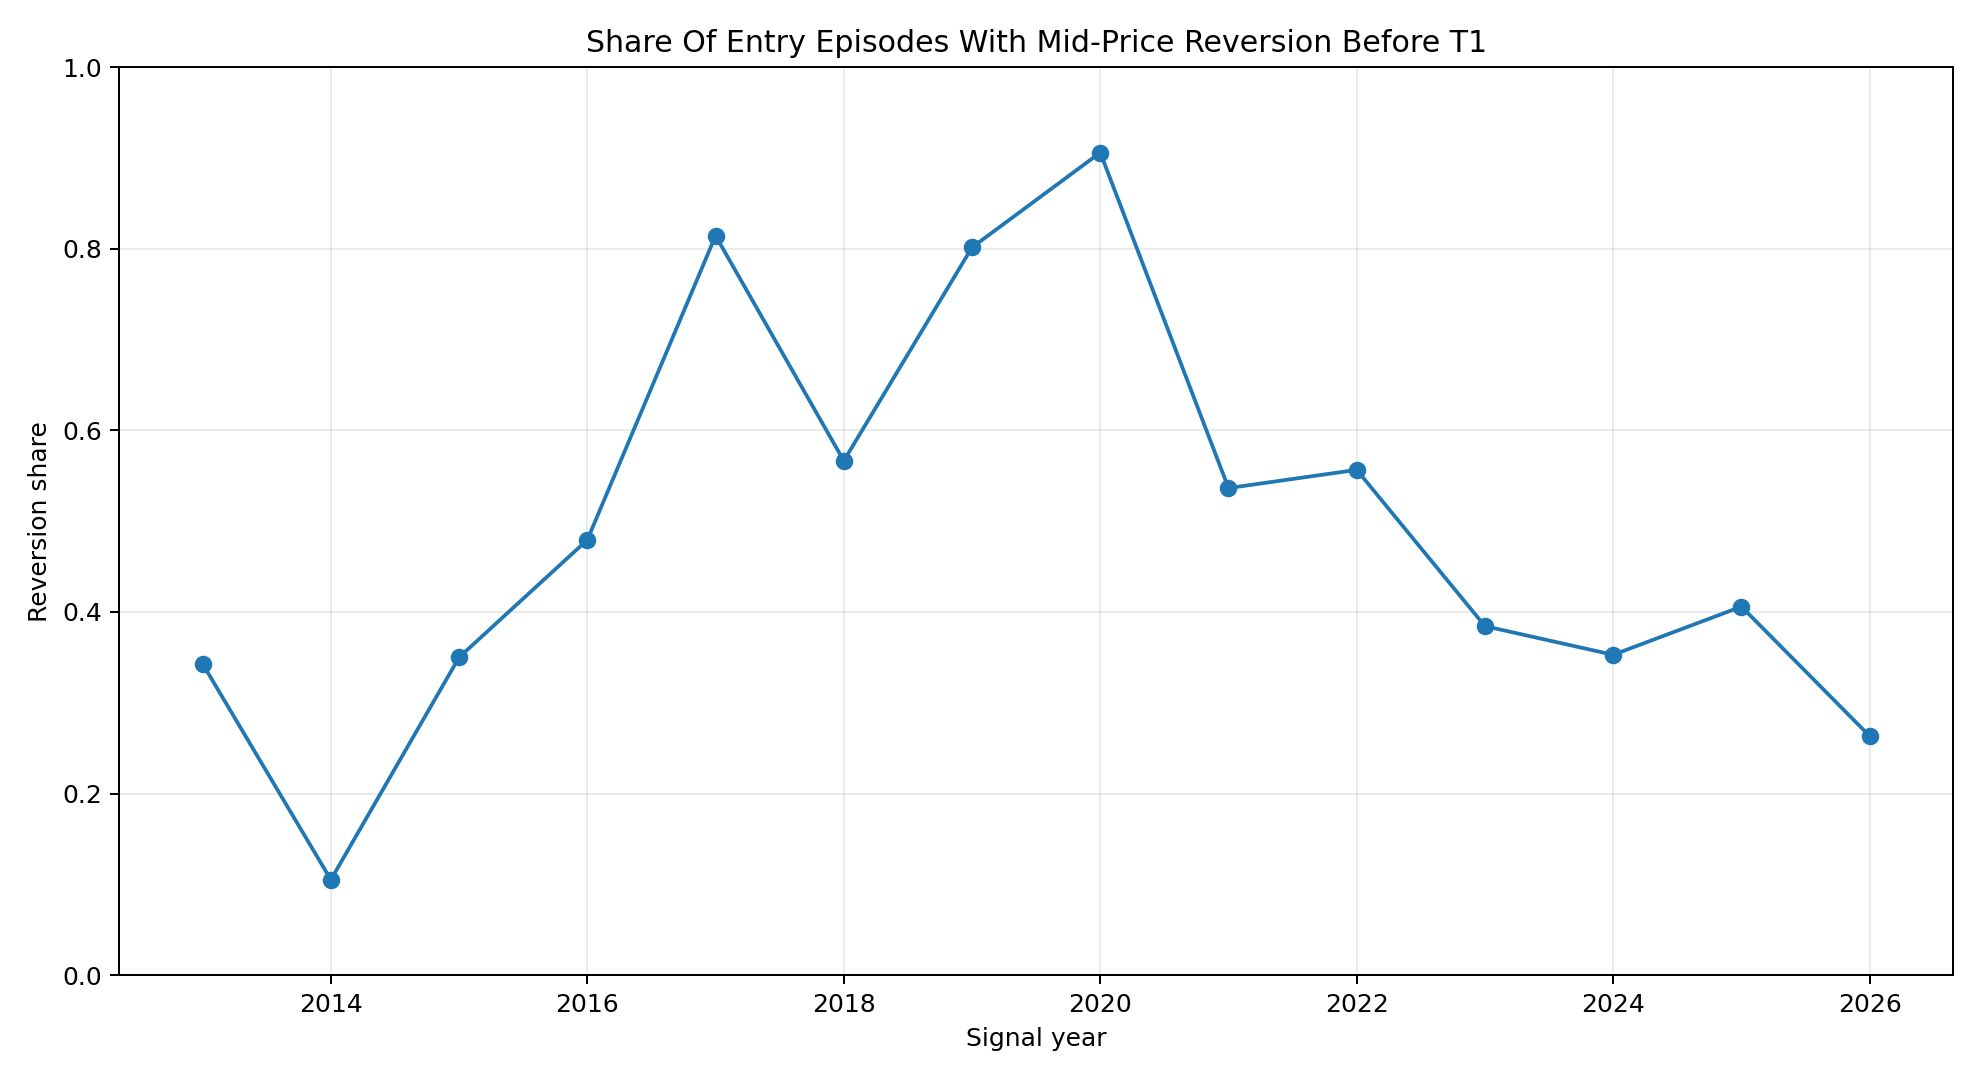
\includegraphics[width=0.92\linewidth]{figures/liquid_exit_reversion_share_by_year.png}
  \caption{Share of entry episodes with a mid-price reversion before T1 expiration.}
  \label{fig:reversion_share}
\end{figure}



\begin{figure}[H]
  \centering
  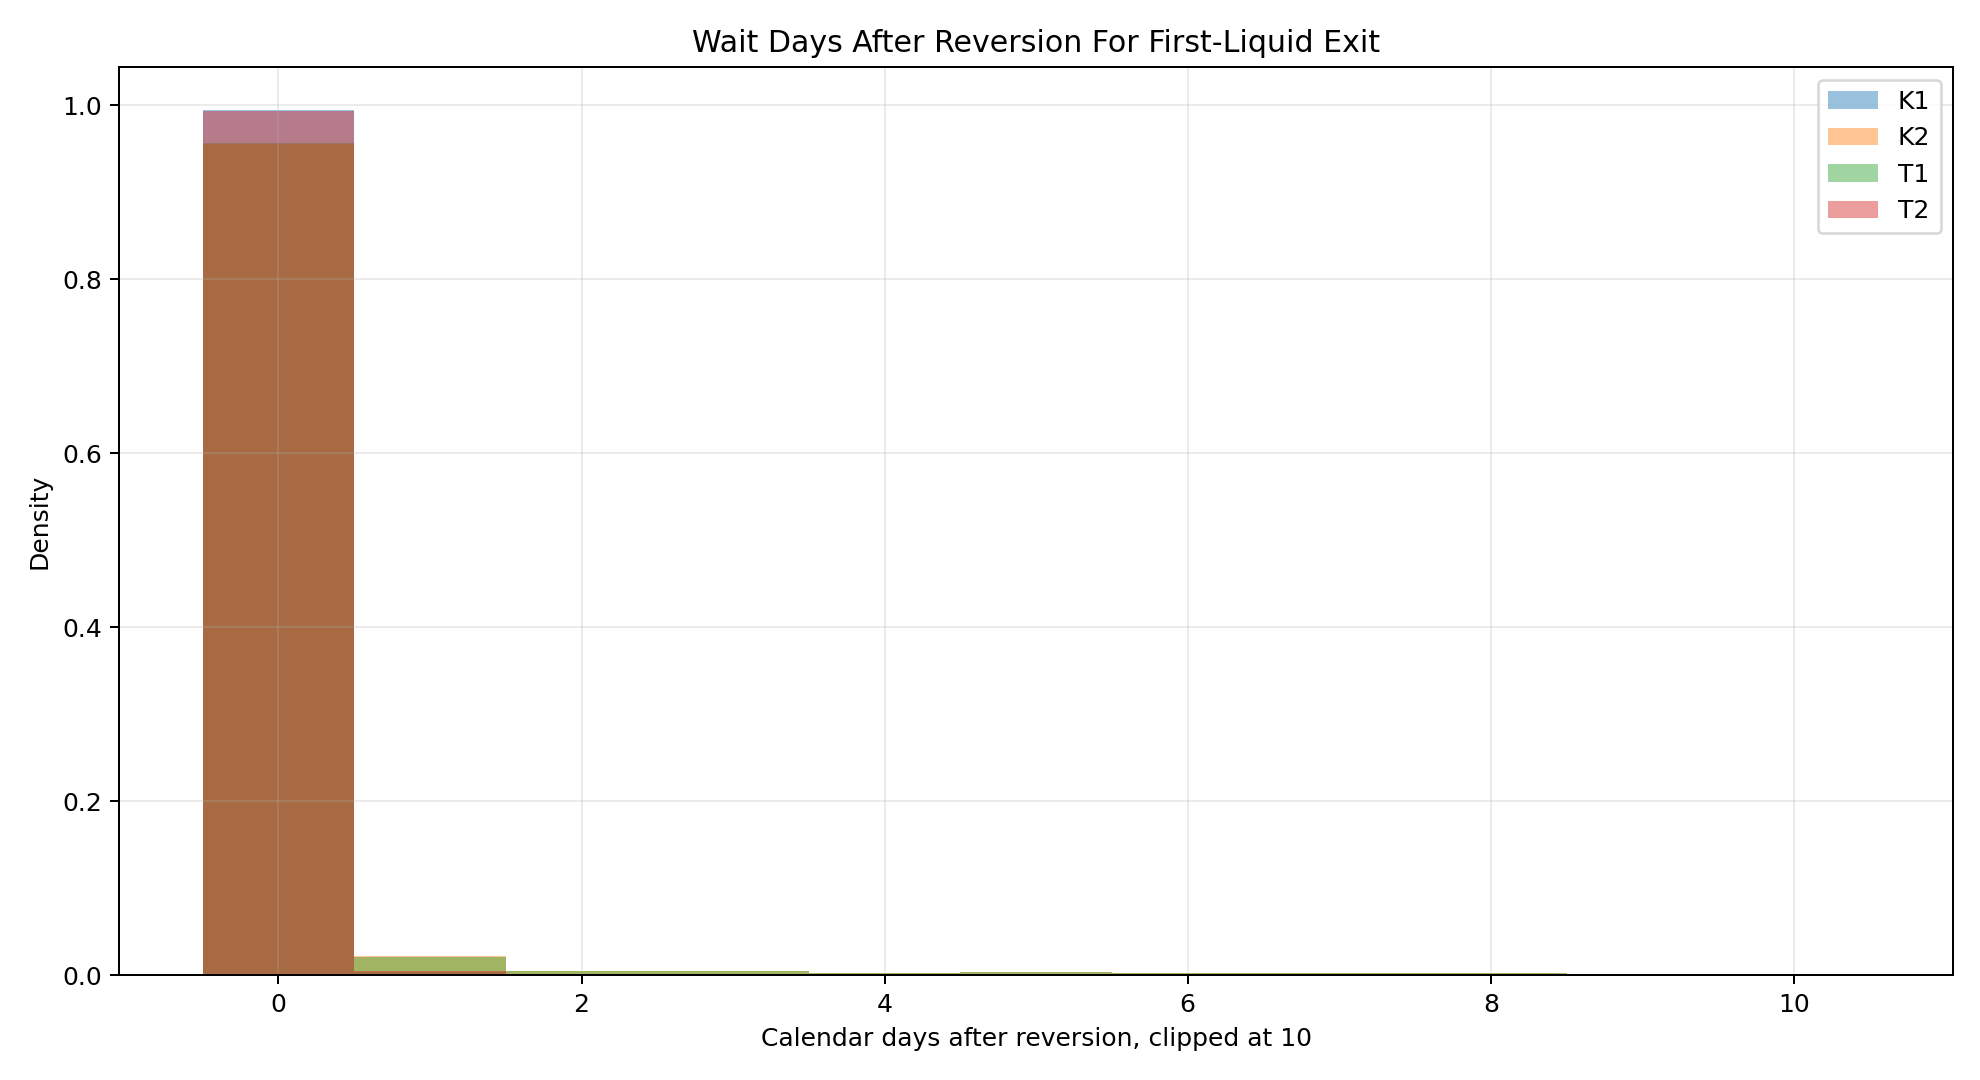
\includegraphics[width=0.92\linewidth]{figures/liquid_exit_wait_days_distribution.png}
  \caption{Wait-time distribution after reversion for first-liquid exit. Most valid exits happen at reversion, with a small but important tail.}
  \label{fig:wait_days}
\end{figure}


\section{How This Becomes ML}

The ML observation unit should be:

\begin{quote}\small
\texttt{episode\_id + strategy + exit\_policy}
\end{quote}

Features must be available at entry time only: entry severity, bid/ask severity, spreads, volume,
open interest, DTE, term gap, moneyness, delta if available, and pre-event lifecycle pressure
features from days \(\le 0\). The model must not use first reversion date, future liquidity, exit
date, realized P\&L, or end-state labels as inputs.

The target can be binary profitability, realized return, or a finite action choice over strategy and
exit policy. The best publishable framing is not ``AI detects arbitrage.'' The stronger framing is:
TP2 gives a theoretically motivated anomaly candidate, and ML learns which tradable episodes,
strategy denominations, and exit policies are economically useful.

\section{Current Interpretation}

\begin{itemize}
  \item The liquid-exit correction is conceptually right: it separates TP2 reversion from immediate
  exit liquidity.
  \item The correction increases executable rows compared with strict reversion-day exit.
  \item T1 and K1 remain the main aggregate premium-resale candidates.
  \item Fixed delays after reversion reduce aggregate P\&L, so waiting blindly is not attractive.
  \item Expiration payoff remains useful as a benchmark, but it should not be mixed with premium
  resale labels in the ML target without explicitly defining the action space.
\end{itemize}

\section{Generated Files}

\begin{quote}\small
\texttt{scripts/build\_liquid\_exit\_labels.py}\\
\texttt{scripts/generate\_liquid\_exit\_latex\_report.py}\\
\texttt{data/labels/archive2\_liquid\_exit\_strategy\_labels\_2013\_2026.parquet}\\
\texttt{data/labels/archive2\_liquid\_exit\_strategy\_labels\_summary\_2013\_2026.json}\\
\texttt{reports/liquid\_exit\_rebuild\_report.pdf}\\
\texttt{reports/raw\_archive2\_eda/tables/liquid\_exit\_rebuild/}\\
\texttt{reports/figures/liquid\_exit\_*.png}
\end{quote}

\end{document}
